%%%%%%%%%%%%%%%%%%%%%%%%%%%%%%%%%%%%%%%%%%%%%%%%%%%%%%%%%%%%%%%%%%%%%%%%%%%%%%%%
%2345678901234567890123456789012345678901234567890123456789012345678901234567890
%        1         2         3         4         5         6         7         8

\documentclass[a4paper, 10pt]{article}
\usepackage[a4paper, margin={2.5cm, 2.5cm}]{geometry}

% The following packages can be found on http:\\www.ctan.org
%\usepackage{epsfig} % for postscript graphics files
%\usepackage{mathptmx} % assumes new font selection scheme installed
%\usepackage{times} % assumes new font selection scheme installed
\usepackage{listings}
\usepackage{graphics}
\usepackage{amsmath}
\usepackage{amssymb}
\usepackage{acro}
\usepackage{enumitem}
\usepackage{graphicx}
\usepackage{wrapfig}
\usepackage{hyperref}
\usepackage{tabularx}
\usepackage{setspace}
\usepackage{comment}
\usepackage{mathrsfs}
\usepackage{tikz}
\usepackage{authblk}

\usepackage{color} %use color
\definecolor{mygreen}{rgb}{0,0.6,0}
\definecolor{mygray}{rgb}{0.5,0.5,0.5}
\definecolor{mymauve}{rgb}{0.58,0,0.82}
\definecolor{pagecolor}{rgb}{1,1,1}
\pagecolor{pagecolor}
%Customize a bit the look
\lstset{ %
backgroundcolor=\color{pagecolor}, % choose the background color; you must add \usepackage{color} or \usepackage{xcolor}
basicstyle=\footnotesize, % the size of the fonts that are used for the code
breakatwhitespace=false, % sets if automatic breaks should only happen at whitespace
breaklines=true, % sets automatic line breaking
captionpos=b, % sets the caption-position to bottom
commentstyle=\color{mygreen}, % comment style
deletekeywords={...}, % if you want to delete keywords from the given language
escapeinside={\%*}{*)}, % if you want to add LaTeX within your code
extendedchars=true, % lets you use non-ASCII characters; for 8-bits encodings only, does not work with UTF-8
frame=single, % adds a frame around the code
keepspaces=true, % keeps spaces in text, useful for keeping indentation of code (possibly needs columns=flexible)
keywordstyle=\color{blue}, % keyword style
% language=Octave, % the language of the code
morekeywords={*,...}, % if you want to add more keywords to the set
numbers=left, % where to put the line-numbers; possible values are (none, left, right)
numbersep=5pt, % how far the line-numbers are from the code
numberstyle=\tiny\color{mygray}, % the style that is used for the line-numbers
rulecolor=\color{black}, % if not set, the frame-color may be changed on line-breaks within not-black text (e.g. comments (green here))
showspaces=false, % show spaces everywhere adding particular underscores; it overrides 'showstringspaces'
showstringspaces=false, % underline spaces within strings only
showtabs=false, % show tabs within strings adding particular underscores
stepnumber=1, % the step between two line-numbers. If it's 1, each line will be numbered
stringstyle=\color{mymauve}, % string literal style
tabsize=2, % sets default tabsize to 2 spaces
title=\lstname % show the filename of files included with \lstinputlisting; also try caption instead of title
}
%END of listing package%
 
\definecolor{darkgray}{rgb}{.4,.4,.4}
\definecolor{purple}{rgb}{0.65, 0.12, 0.82}
 

%define Javascript language
\lstdefinelanguage{JavaScript}{
keywords={typeof, new, true, false, catch, function, return, null, catch, switch, var, if, in, while, do, else, case, break},
keywordstyle=\color{blue}\bfseries,
ndkeywords={class, export, boolean, throw, implements, import, this},
ndkeywordstyle=\color{darkgray}\bfseries,
identifierstyle=\color{black},
sensitive=false,
comment=[l]{//},
morecomment=[s]{/*}{*/},
commentstyle=\color{purple}\ttfamily,
stringstyle=\color{red}\ttfamily,
morestring=[b]',
morestring=[b]"
}
 
\lstset{
language=JavaScript,
extendedchars=true,
basicstyle=\footnotesize\ttfamily,
showstringspaces=false,
showspaces=false,
numbers=left,
numberstyle=\footnotesize,
numbersep=9pt,
tabsize=2,
breaklines=true,
showtabs=false,
captionpos=b
}
%---------------------------------------------------
%----- Hyper Setup
%---------------------------------------------------
\hypersetup{
	pdftitle={Centrifuge:  Protocol for private by design transactions on a decentralized network}, 
    pdfauthor={Lucas Vogelsang,Manuel Polzhofer, Philip Stehlik,Miguel Hervas Lazaro}, 
    pdfsubject={Protocol Paper, Centrifuge}, % please, select the type of this document
    pdfstartview={FitH},    % fits the width of the page to the windowhttps://www.overleaf.com/project/5c35d0fa8c97d86e2adb91c2
    pdfnewwindow=true, 		% links in new window
    colorlinks=true,  		% false: boxed links; true: colored links
    linkcolor=orange,          % color of internal links
    citecolor=orange,        % color of links to bibliography
    filecolor=magenta,      % color of file links
    urlcolor=black           % color of external links
}
% 


\makeatletter
\newcommand*{\xleftrightarrow}[2]{\mathrel{
  \settowidth{\@tempdima}{$\scriptstyle#1$}
  \settowidth{\@tempdimb}{$\scriptstyle#2$}
  \ifdim\@tempdimb>\@tempdima \@tempdima=\@tempdimb\fi
  \mathop{\vcenter{
    \offinterlineskip\ialign{\hbox to\dimexpr\@tempdima+1em{##}\cr
    \rightarrowfill\cr\noalign{\kern.5ex}
    \leftarrowfill\cr}}}\limits^{\!#1}_{\!#2}}}


%---------------------------------------------------
%----- Version
%---------------------------------------------------
\def\ProtocolPaperVersionNumber{unknown revision}
\IfFileExists{Options.tex}{\input{Options.tex}}

%---------------------------------------------------
%----- Helper Commands
%---------------------------------------------------
\newcommand{\codesection}[1]{\doublespacing{\hspace{\parindent}\texttt{#1}}}
\newcommand{\sbline}{\\[.5\normalbaselineskip]}% small blank line 
\newcommand{\ethleftarrow}{\ensuremath{\xleftarrow[]{\text{ETH}}}}


\title{\LARGE \bf
Centrifuge: Protocol for private by design transactions on a decentralized network
}
\date{\ProtocolPaperVersionNumber}
\author{Lucas Vogelsang\thanks{Lucas Vogelsang, {\tt\small l@lucasvo.com}} \hspace{0.1cm} Manuel Polzhofer\thanks{Manuel Polzhofer, {\tt\small manuel@centrifuge.io}}  \hspace{0.1cm} Philip Stehlik\thanks{Philip Stehlik, {\tt\small philip@centrifuge.io}} \hspace{0.1cm} Vimukthi Wickramasinghe\thanks{Vimukthi Wickramasinghe, {\tt\small vimukthi@centrifuge.io}} 
\newline Miguel Hervas Lazaro\thanks{Miguel Hervas Lazaro, {\tt\small miguel@centrifuge.io}}}


%%%%%%%%%%%%%%%%%%%%%%%%%%%%%%%%%%%%%%%%%%%%%%%%%%%%%%%%%%%%%%%%%%%%%%%%%%%%%%%%
\acsetup{first-style=short}

\begin{document}

\maketitle
\thispagestyle{empty}
\pagestyle{empty}

%---------------------------------------------------
%----- Content
%---------------------------------------------------
\input{abstract}
\input{1_introduction}
\input{2_high_level}
\input{3a_document_fields}
%---------------------------------------------------
%----- Version History
%---------------------------------------------------
\subsubsection{Version History}\label{sec:version_history}
The version history $H$ is a set of documents. An update of an existing document in the Centrifuge protocol happens by creating a new version and linking this new version to the previously existing version. 
We define the set of all documents as $D$:
\begin{equation}
d \in D
\end{equation}
Every node keeps a history of all versions of a document in which they are listed as a collaborator.
\begin{equation}
H = (d_{[0]},...,d_{[n]})
\end{equation}
\newline
In the initial version of a document $d_0$, the current version and the identifier will be equal.
\begin{equation}
d_{[0]{\texttt{id}}} = d_{[0]\texttt{current}}
\end{equation}
\newline
The fields for the previous document root hash $D_{\texttt{prev-root}}$ and for the $D_{\texttt{prev}}$ id will be empty in the initial version.
\begin{eqnarray}
d_{[0]{\texttt{prev-root}}}& = & \emptyset \\
d_{[0]{\texttt{prev}}} & = & \emptyset
\end{eqnarray}
\newline
For all other documents $D$ in a version history $H$, the following conditions must be true:
\newline
\newline
Every document in a version history $H$ must have the same identifier.
\begin{equation}
\{d_{[i]} \in H \mid \forall d_{[j]} \in H :d_{[i]\texttt{id}} = d_{[j]\texttt{id}} \}
\end{equation}
\newline
The current version field of a document must be equal to the next version field of the previous document.
\begin{equation}
d_{[i]\texttt{current}} = d_{[i-1]\texttt{next}} 
\end{equation}
\newline
The previous version field of a document must be equal to the current version field of the predecessor document.
\begin{equation}
d_{[i]\texttt{prev}} = d_{[i-1]\texttt{current}} 
\end{equation}
\newline
The previous root hash of a document must be equal to the document root hash of the predecessor document.
\begin{equation}
d_{[i]\texttt{prev-root}} = d_{[i-1]\texttt{doc-root}}
\end{equation}
\newline
The current pre-image of a document must be equal to the next pre image of the predecessor document.
\begin{equation}
d_{[i]\texttt{current-img}} = d_{[i-1]\texttt{next-img}}
\end{equation}
\newline
The history of the document can therefore be seen as a doubly linked list. Every document has the document hash $d_{\texttt{previous}}$ of the predecessor document and defines the $d_{\texttt{id}}$ of the next one.\\\\
A node which performs a document update defines the the next version identifier $d_{\texttt{next}}$.
\begin{equation}
d_{[i]\texttt{next-img}} = \texttt{RAND(32)}
\end{equation}
\begin{equation}
d_{[i]\texttt{next}} = \mathtt{blake2b}(d_{[i]\texttt{next-img}})
\end{equation}
\newline
The field $d_{\texttt{next-img}}$ is needed to prevent malicious anchoring of documents by non-collaborators. The value therefore must be kept secret from any non-collaborators. The function $\texttt{RAND(32)}$ is a cryptographically secure random function and returns a byte 32 array. The function $\mathtt{blake2b}$ denotes hash function blake2b-256. 

By referencing the previous root each state $d$, the history becomes an immutable attribute committed to in each version. To traverse the history $H$, one can follow the $d_{\mathtt{prev-root}}$ and $d_{\mathtt{prev}}$. To move forward in the list of history, $H$, one can go from $d_{\mathtt{next}}$ to $d_{\mathtt{current}}$.
\begin{figure}[thpb]
  \centering
  \includegraphics[width=16cm]{img/documents-history-v2.png}
  \caption{Doubly linked list of different versions of a document. Indicating the relationship between different document index fields. The document root $R_{\texttt{doc-root}}$ is stored in the anchor registry and not in the document itself.} 
  \label{fig:documents}
\end{figure}


%---------------------------------------------------
%----- Calculation of the Root Hashes
%---------------------------------------------------
\subsection{Calculation of the Root Hashes}
Every root hash of a document $R_{\texttt{doc-root}}$ is stored in the
\textit{AnchorRepository} smart contract. The document root hash is calculated from three different Merkle trees (see Fig. \ref{fig:root-hash}). 
\subsubsection{Merkle Tree of Fields}
A Merkle tree is a way to calculate a unique hash from a set of items. We formally define a Merkle tree function $\mathcal{M}$ to calculate a root hash $R \in \mathbb{B}_{32}$ of document fields $F$. The implementation of the Merkle tree function is introduced in Sec. \ref{sec:precise_proofs}.
 \begin{eqnarray}
 R & = &\mathcal{M}(F_{[0]},...,F_{[n]}) \\
 R & \in & \mathbb{B}_{32}
\end{eqnarray}
\newline
\subsubsection{Model Merkle tree}
As a first step, we calculate the Merkle tree of the schema fields $S$ and the core document fields $C$ of a document $d$.\\
As a second step, we flatten and combine all leaves from each tree.\\ 
Finally, we calculate the Model Merkle Root\\\\
\textbf{Model Root} The Merkle root of the flattened document schema and the core document data, formally $R_{{\texttt{model}}}$ 
\newline
\begin{equation}
    d_M = (d_S \cup d_C)
\end{equation}
\begin{equation}
    R_{{\texttt{model}}} = \mathcal{M}(d_M)
\end{equation}
\newline
 \subsubsection{Basic and ZK Model trees}
\textbf{Basic Model} The Merkle tree of the flattened document schema and the core document data, formally $R_{{\texttt{basic-model}}}$
\newline
\begin{equation}
    R_{{\texttt{basic-model}}} = \mathcal{M}(d_{MB})
\end{equation}
\newline
The Basic Model tree has the following properties:
\begin{itemize}  
\item Leaf Hashing function keccak-sha3 (add ref) of 256 bits
\item Node Hashing function blake2b (add ref) of 256 bits
\item Sorted Hashes
\end{itemize}
\newline
\textbf{ZK Model} The Merkle tree of the flattened document schema and the core document data ready for Zero Knowledge proving, formally $R_{{\texttt{zk-model}}}$
\newline
\begin{equation}
    R_{{\texttt{zk-model}}} = \mathcal{M}(d_{MZ})
\end{equation}
\newline
The ZK Model tree has the following properties:
\begin{itemize}  
\item Leaf Hashing function keccak-sha3 of 256 bits
\item Node Hashing function pedersen (add ref) of 256 bits
\item Ordered (Left-Right) Hashes
\item Fixed size of 20 levels
\end{itemize}
 \subsubsection{Signing Root}
The $R_{\texttt{signing}}$ is calculated from the blake2b-256 hash of the concatenated $R_\texttt{basic-model}$ and $R_{\texttt{zk-model}}$
\newline
\begin{equation}
R_{\texttt{signing}} = \texttt{blake2b}(R_\texttt{basic-model}\| R_{\texttt{zk-model}})
\end{equation}\\
We formally define a helper function for calculating the $R_{\texttt{signing}}$ 
\begin{eqnarray}
R_{\texttt{signing}}& =&\mathsf{calculateSigningRoot}(d) \\
\mathsf{calculateSigningRoot}(d)& =& \texttt{blake2b}(\mathcal{M}(d_{MB})\| \mathcal{M}(d_{MZ}))
\end{eqnarray}
 \subsubsection{Signatures Root}
 A Merkle root of the collaborator signature must be part of the document root hash $R_{\texttt{doc-root}}$. The signatures are relevant for the document consensus, explained in the following chapters. \\\\
\textbf{Signature Root} A signature root hash defines the Merkle root of all signatures $d_{\texttt{signatures}}$, formally $R_{\texttt{signatures}}$:
\newline
\begin{equation}
R_{\texttt{signatures}} = \mathcal{M}(d_{\texttt{signatures}})\\
\end{equation}
 \subsubsection{Document Root}
The final  document root hash $R_{\texttt{doc-root}}$ of the entire document $d$ is defined as the blake2b hash of the concatenated signing root hash $R_{\texttt{signing}}$ and signature root hash $R_{\texttt{signatures}}$ 
\newline
 \begin{equation}
R_{\texttt{doc-root}} =  \texttt{blake2b}(R_{\texttt{signing}}\|R_{\texttt{signatures}})
\end{equation}\\
A tree of the  $R_{\texttt{doc-root}}$ calculation. (see Fig. \ref{fig:root-hash})

%TODO (Manuel): Why sometimes R and D?

%All information related to the document is stored in a structured protobuf message called CoreDocument, \mathsf{CD}, along with a document-specific message, Data, \mathsf{D} such as an Invoice or PurchaseOrder. Both messages are serialized with precise proofs into \\mathsf{CD} 

\begin{figure}[thpb]
\centering
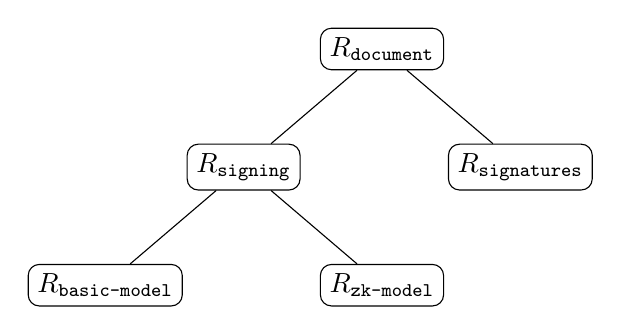
\begin{tikzpicture}[sibling distance=10em,
  every node/.style = {shape=rectangle, rounded corners,
    draw, align=center, %top color=white, bottom color=gray!20
    }]]
  \node {$R_{{\texttt{document}}}$}
    child { node {$R_{{\texttt{signing}}}$}  child { node {$R_{{\texttt{basic-model}}}$}  
    } child { node {$R_{{\texttt{zk-model}}}$} 
    } }
    child { node {$R_{{\texttt{signatures}}}$}};
\end{tikzpicture}
\caption{Calculation of the last layers of the document merkle tree. The leafs are the roots of merkle trees from the different document parts }\label{fig:root-hash}
\end{figure}
We can define a second help function called $\mathsf{calculateDocumentRoot}(d)$ for calculating the entire $R_{\texttt{doc-root}}$. 
\begin{eqnarray}
R_{\texttt{doc-root}}& =&\mathsf{calculateDocumentRoot}(d) \\
\mathsf{calculateDocumentRoot}(d)& = & \texttt{blake2b}( \mathsf{R_{\texttt{signing}}}\| \mathcal{M}_{\texttt{tree}}(d_S))
\end{eqnarray}
\input{3d_state_commit}
\input{3e_protobufsproofs}
\input{4_participants}
\input{5_consensus}
\input{6_transitions}
\input{7_wire_protocol}
\input{8_nft}
\input{9_versions}


%---------------------------------------------------
%----- Bibliography
%---------------------------------------------------
\phantomsection
\addcontentsline{toc}{chapter}{Literature}
\bibliographystyle{plain}
\bibliography{references.bib}



%\printacronyms[include-classes=nomencl,name=Nomenclature]
%\printacronyms[include-classes=abbrev,name=Abbreviations]
\input{appendix}

\end{document}

